\documentclass[../main.tex]{subfiles} % Import document.
\begin{document}
\subsection{Opgave 5}
"for"-løkken løber igennem listen L og læser, hvor kanten går fra (L[j][1]) og sætter den værdi til -1 til den pågældende kant j. Derefter læser den, hvor kanten går til og sætter værdien lig 1.

\subsection{Opgave 6}
BFS!
\subsection{Opgave 7}
Der tilføjes netop én kant når der tilføjes et nyt punkt
\subsection{Opgave 8}

    \begin{figure}[H]
		\centering
		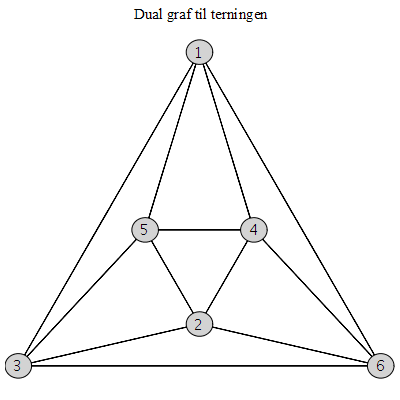
\includegraphics[width=0.5\linewidth]{images/opg8DualGraf.png}
		\caption[]{Dual Graf}
		\label{fig:opg8DualGraf}
    \end{figure}

\end{document}